\chapter{Multi Layer Perceptron và Deep Learning}
\label{chp:03}

\section{Logistic regression dưới góc nhìn neural network}
\label{sec31}
\textit{Hồi quy logistic} (logistic regression) là một \textit{phương pháp phân loại nhị phân} (binary classification method), được xây dựng bởi một hàm có khả năng nhận một giá trị bất kỳ và trả kết quả ra một con số nằm giữa 0 và 1 (hàm sigmoid). Điều này cũng tương tự như một \textit{mạng nơ-ron} (neural network) một lớp. Hình \ref{fig:LogisticRegressionNN} minh họa cho việc dùng hồi quy logistic như một mạng nơ-ron đơn giản.

\begin{figure}[!h]
	\centering
		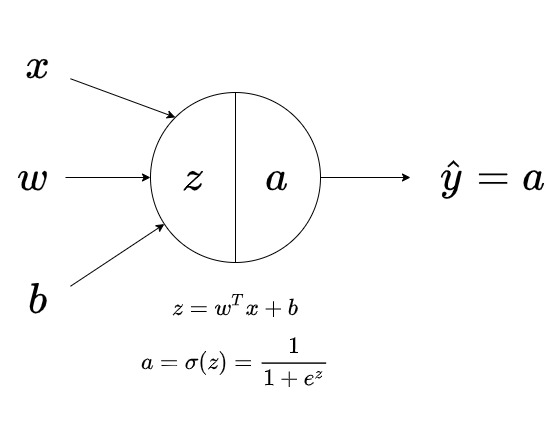
\includegraphics[width=0.5\columnwidth]{chapter03/figure/LogisticRegressionNN.jpg}
        \caption{Một mạng nơ-ron đơn giản.}
        \label{fig:LogisticRegressionNN}
		\centering
\end{figure}

Trong hình \ref{fig:LogisticRegressionNN}, ma trận $x$ chứa các \textit{thuộc tính} (feature) của một input, ma trận $w$ sẽ là trọng số các thuộc tính và $b$ là bias. Sau khi trải qua các bước tính toán, kết quả thu được $\hat{y}$ sẽ là xác suất \textit{nhãn} (label) $y$ nhận giá trị bằng 1 với $x$ và $w$ đã biết.
\[ P(y=1|w,x) = \hat{y}\]

Như đã trình bài ở trên, kết quả của hàm $\sigma$ luôn là một giá trị từ 0 đến 1. Nhưng giá trị của nhãn thì luôn là 0 hoặc 1. Sự sai biệt này dẫn đến khái niệm \textit{hàm mất mát} (loss function). Có rất nhiều hàm có thể được dùng để làm hàm mất mát, tuy nhiên trong chương này ta sẽ chỉ dùng \textit{ hàm mất mát Cross-entropy} (Cross-entropy loss function) được định nghĩa như sau.
\[ L(\hat{y},y) = -  [y\log{\hat{y}} + (1-y)\log{(1-\hat{y})}] \]

Giá trị của hàm mất mát là kết quả của \textit{lan truyền xuôi} (forward propagation) và đóng vai trò then chốt trong quá trình \textit{lan truyền ngược} (backward propagation).

\begin{figure}[!h]
	\centering
		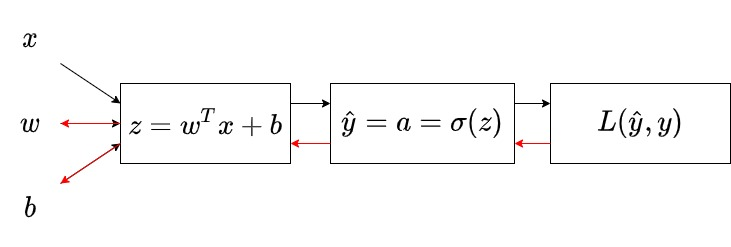
\includegraphics[width=0.5\columnwidth]{chapter03/figure/Back-fowardPropagation.jpg}
        \caption{Lan truyền xuôi và lan truyền ngược.}
        \label{fig:backfowardPropagation}
		\centering
\end{figure}

Quan sát hình \ref{fig:backfowardPropagation}, quá trình lan truyền ngược và cập nhật trọng số bằng \textit{gradient descent} được thực hiện như sau (giả sử $w$ có kích thước $1\times n$):

1.$\indent $ Tính đạo hàm riêng phần của $L(\hat{y},y)$ theo $w_i$ (với $i=1...n$).
    \begin{align*}
        \frac{\partial L}{\partial w_i} &= \frac{\partial L}{\partial a}\times\frac{\partial a}{\partial w_i } \\
        &= \frac{\partial L}{\partial a}\times \frac{\partial a}{\partial z} \times \frac{\partial z}{\partial w_i}\\
        &= (\frac{1-y}{1-a}-\frac{y}{a})\times \frac{\partial a}{\partial z} \times \frac{\partial z}{\partial w_i}\\
        & = (\frac{1-y}{1-a}-\frac{y}{a}) \times a \times (1-a)\times \frac{\partial z}{\partial w_i}\\
        & =  (\frac{1-y}{1-a}-\frac{y}{a}) \times a \times (1-a)\times x_i\\
        &= (a-y) \times x_i\\
        &= (\hat{y}-y) \times x_i
    \end{align*}

2.$\indent$ Cập nhật lại trọng số bằng gradient descent:
\begin{align*}
    w_i &= w_i - \alpha \times \frac{\partial L}{\partial w_i}\\
    &= w_i - \alpha \times(\hat{y}-y) \times x_i
\end{align*}

Cách cập nhật trọng số được trình bày ở trên xét trên mà trên $x$ có kích thước $1\times n$. Trường hợp $x$ có kích thước $m \times n$, ta sẽ áp dụng gradient descent với $\frac{\partial J}{\partial w_i}$ thay vì $\frac{\partial L}{\partial w_i}$. Trong đó, J là \textit{cost} được tính theo công thức sau (với $y^{(i)}$ và  $\hat{y}^{(i)}$ lần lượt là nhãn và kết quả dự đoán của $x^{i}$):
\[J = -\frac{1}{m} \times \sum_{i=1}^{m}L(\hat{y}^{(i)},y^{(i)})\]
%%%%%%%%%%%%%%%%%%%%%%%%%%%%%%%%%%%%%%%%%%%%%%%%%%%%%%%%%%

\section{Mạng neural network nhiều lớp(MLP) và mạng học sâu}
\subsection{Nhắc lại mạng neural network nhiều lớp}
Như chương trước đã đề cập, mạng neural network nhiều lớp thực chất chỉ gồm nhiều tầng mà trong mỗi tầng các perceptron đặt chồng lên nhau. Cách thức hoạt động của những tầng mạng cũng rất đơn giản bằng cách nhân ma trận. Bằng cách này, chúng ta có thể giải quyết rất nhiều bài toán. Tuy nhiên, khi để ý thì tất cả các phép tính này đều xây dựng trên hàm tuyến tính. Điều này gây ra những vấn đề sau:
\begin{itemize}
    \item Khó khăn trong việc xây dựng những mô hình phi tuyến phức tạp.
    \item Khi đi qua nhiều lớp, những vấn đề về trọng số sẽ xảy ra ví dụ như đầu ra của một perceptron nào đó quá lớn hoặc quá âm sẽ ảnh hưởng rất nhiều đến độ chính xác của bài toán hoặc thậm chí là máy tính không thể biểu diễn được.
    \item Vì đầu ra sẽ được so sánh về ngưỡng nào đó, do đó, vấn đề về xác định xác suất sẽ rất khó thực hiện vì chúng ta chỉ thể hiện được mức độ hay nói cách khác là những giá trị rời rạc. Ví dụ như chúng ta muốn nhận diện chó hoặc mèo, thì mô hình xây dựng trên MLP chỉ cho phép ta biết đó là chó hoặc mèo chứ không cho ta biết xác suất mà mô hình nhận diện được vật thể đó là chó là bao nhiêu phần trăm.
\end{itemize}

\subsection{Sự tiến hóa của mạng neural netwwork nhiều lớp}
Sau những vấn đề được nêu ra ở trên thì chúng ta thấy rằng, vấn đề đang nằm ở hàm activation và nó cần được thay đổi. Nhưng thay đổi làm sao và thế nào lại là một câu hỏi khó.

Không sao cả, vấn đề chỗ nào thì chúng ta sẽ đi gỡ rối chỗ đó tương ứng như sau. 
\begin{itemize}
    \item Do việc xây dựng MLP như trên đang theo mô hình tuyến tính đối với 2 tầng gần nhau. Do đó, dễ nghĩ đến là chúng ta sẽ thiết kế một hàm activation phi tuyến. (1)
    \item Khi đi qua nhiều lớp, những vấn đề về trọng số sẽ xảy ra ví dụ như đầu ra của một perceptron nào đó quá lớn hoặc quá âm sẽ ảnh hưởng rất nhiều đến độ chính xác của bài toán. Để giải quyết điều này, chúng ta sẽ đi tìm hàm sao cho có thể kéo những giá trị đầu ra về 1 khoảng nào đó có thể kiểm soát được và có ý nghĩa trong xác suất thống kê như (-1,1) hoặc (0,1). (2)
    \item Vấn đề thể hiện độ tin cậy mà mô hình cho ra sẽ cho chúng ta ý tưởng về thiết kế hàm activation sao cho kết quả cho ra nằm trong khoảng (0,1) thể hiện cho xác suất. (3) 
\end{itemize}

Từ (1),(2),(3) chúng ta sẽ thiết kế hàm activation sao cho đó là hàm phi tuyến (hàm này sẽ phải có đạo hàm) và đầu ra nên có giá trị (-1,1) hoặc (0,1).

Sau một thời gian phát triển, các mạng học sâu đã ra đời và dựa trên những hàm activation này.

\subsection{Mạng học sâu}
Bằng cách áp dụng các hàm activation khác nhau thay cho threshold và cách làm tuyến tính như MLP thì mạng học sâu đã ra đời. Chúng ta cũng dễ thấy rằng, không có sự khác biệt quá nhiều giữa MLP và mạng học sâu (như hình minh họa) hay có thể nói MLP là một tập hợp con của mạng học sâu khi chúng ta chỉ cần thay đổi activation của từng hidden layers và layer đầu ra để thể hiện về tính phi tuyến và xác suất.

\begin{figure}[!h]
	\centering
		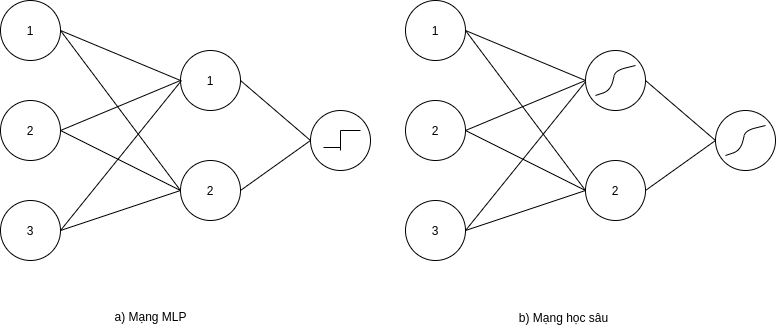
\includegraphics[width=10cm, height=5cm]{chapter03/figure/neuralnetwork.png}
        \caption{Hình a) miêu tả mạng MLP với 1 hidden layer, hình b) miêu tả mạng học sâu với 1 hidden layer}
        \label{fig:neuralnetwork}
		\centering
\end{figure}

Như hình trên, chúng ta có thể thấy rằng, đi qua mỗi layer của mạng học sâu chúng ta có thể thêm vào đó các hàm activation khác nhau, hoặc thậm chí không cần thêm. Còn trong MLP thì chỉ đơn thuần là các phép tính toán ma trận tuyến tính.

\section{Các hàm activation functions}
\subsection{Hàm sigmoid}
$\indent$\textbf{Công thức:}
\[ \sigma(x) = \frac{1}{1+e^{-x}} \]
$\indent$Hàm sigmoid nhận vào một giá trị thực $x$ và trả về một giá trị trong khoảng $(0,1)$. Nếu $x$ là một số thực âm rất nhỏ thì kết quả của hàm sigmoid sẽ tiệm cận 0, và ngược lại nếu $x$ là một số dương rất lớn thì kết quả sẽ tiệm cận 1. Hình \ref{fig:HamSigmoid} bên dưới là đồ thị biểu diễn cho hàm sigmoid.

\begin{figure}[!h]
	\centering
		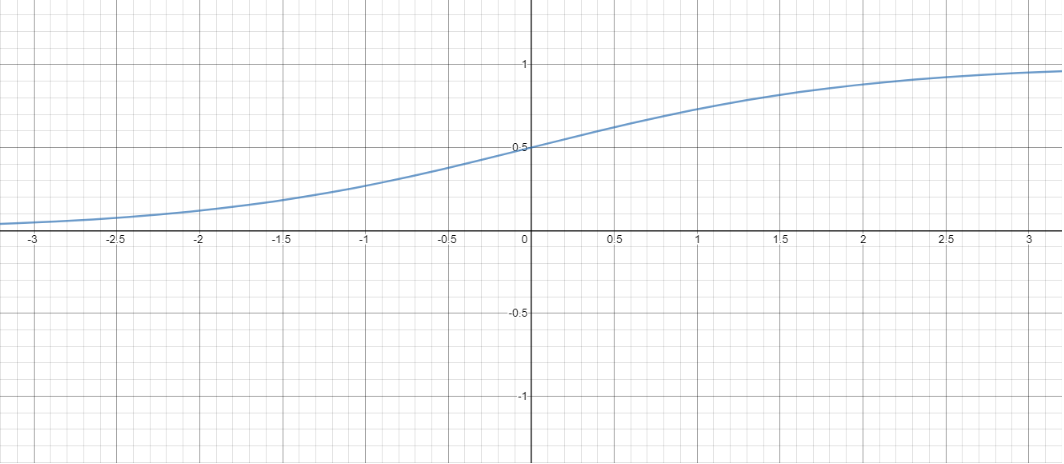
\includegraphics[width=0.75\columnwidth]{chapter03/figure/HamSigmoid.png}
        \caption{Đồ thị của hàm sigmoid.}
        \label{fig:HamSigmoid}
		\centering
\end{figure}

Như đã thấy ở phần \ref{sec31}, khi sử dụng hàm sigmoid làm hàm activation, việc tính toán vô cùng thuận lợi do kết quả đạo hàm của sigmoid rất "đẹp". Tuy nhiên, điều này không thể che lấp những khuyết điểm nghiêm trọng của sigmoid:

\begin{enumerate}
    \item \textbf{Hàm sigmoid bão hòa và \textit{triệt tiêu gradient} (vanishing gradient)}
    \begin{figure}[!h]
	\centering
		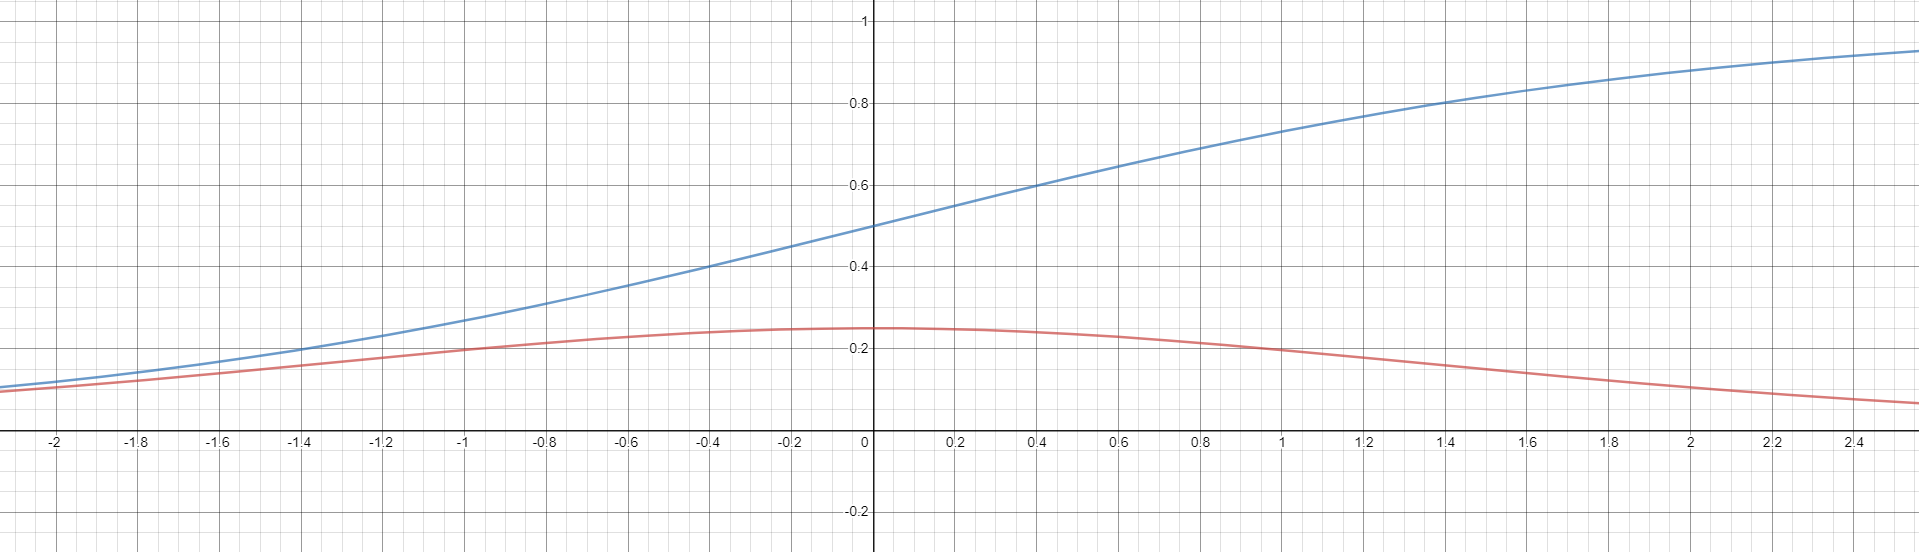
\includegraphics[width=0.75\columnwidth]{chapter03/figure/VanishingGradient.png}
        \caption{Giá trị và đạo hàm của hàm sigmoid.}
        \label{fig:VanishingGradient}
		\centering
    \end{figure}
    
    Trên hình \ref{fig:VanishingGradient}, đường màu xanh thể hiện cho giá trị của hàm sigmoid và đường màu đỏ thể hiện cho giá trị của đạo hàm. Có thể nhận ra được, với những giá trị $x$ rất lớn hoặc rất nhỏ, kết quả đạo hàm của hàm sigmoid rất gần với 0. Điều này gây ra sự triệt tiêu gradient và hạn chế khả năng học của mạng. Cụ thể, nếu mạng được khởi động bằng những trọng số quá lớn hoặc quá nhỏ, giá trị đầu vào của hàm sigmoid bị bão hòa, giá trị của đạo hàm sẽ là một giá trị gần 0 và gradient sẽ bị triệt tiêu. Nếu mạng được khởi động bằng những trọng số "đẹp" (không quá lớn, không quá nhỏ), giá trị của đạo hàm cũng sẽ là một giá trị trong khoảng (0,0.25). Khi đi qua một mạng nhiều tầng, đạo hàm của các trọng số sẽ nhỏ dần và gradient vẫn sẽ bị triệt tiêu.
    \item \textbf{Hàm sigmoid không có tính chất \textit{zero-centered}}
    \begin{figure}[!h]
	\centering
		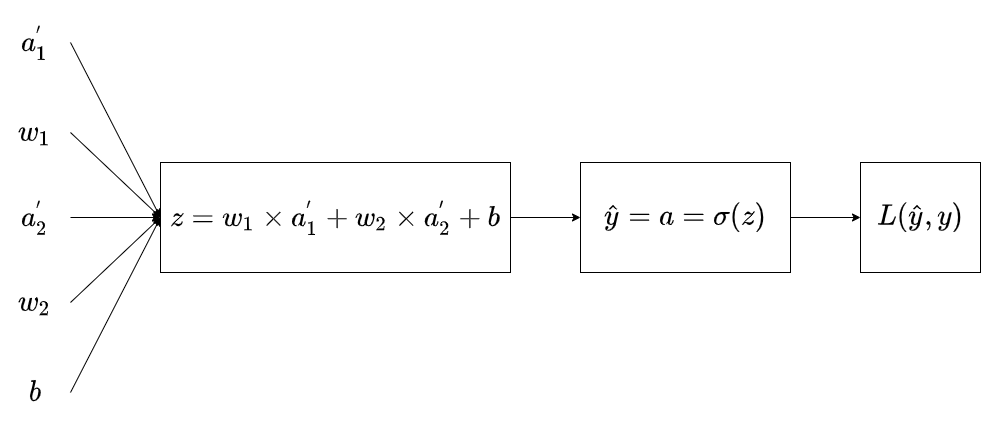
\includegraphics[width=0.5\columnwidth]{chapter03/figure/ZeroCentered.png}
        \caption{Một tầng ẩn của mạng neural nhiều lớp dùng hàm sigmoid.}
        \label{fig:ZeroCentered}
		\centering
    \end{figure}
    
    Ở ví dụ của mạng neuron như Hình \ref{fig:ZeroCentered}, đạo hàm riêng phần của hàm mất mát theo hai trọng số $w_1$ và $w_2$ sẽ được tính như sau:
    \begin{align*}
        \nabla w_{1} &= \frac{\partial L}{\partial z} \times \frac{\partial z}{\partial w_1} = \frac{\partial L}{\partial z} \times a^{'}_1\\
        \nabla w_{2} &= \frac{\partial L}{\partial z} \times \frac{\partial z}{\partial w_2} = \frac{\partial L}{\partial z} \times a^{'}_2
    \end{align*}
    
    Vì $a^{'}_1$ và $a^{'}_1$ là kết quả của một hàm sigmoid trước đó, do đó luôn nhận giá trị dương và dấu của các gradient sẽ phụ thuộc vào $\frac{\partial L}{\partial z}$. Điều này có nghĩa là các gradient sẽ luôn cùng dương hoặc luôn cùng âm. Việc cập nhật trọng số sẽ chỉ xảy ra về một phía, hạn chế sự linh hoạt của mạng và gây khó khăn cho việc hội tụ.
\end{enumerate}

\subsection{Hàm tanh}
$\indent$\textbf{Công thức:}
\[tanh(x) = \frac{e^x-e^{-x}}{e^x+e^{-x}}\]
$\indent$Hàm tanh nhận vào một số thực và trả về một giá trị trong khoảng (-1,1). Trên hình \ref{fig:Tanh}, đường màu xanh thể hiện giá trị của hàm tanh và đường màu đỏ thể hiện cho giá trị đạo hàm. Dễ dàng nhận thấy rằng hàm tanh cũng gặp phải vấn đề triệt tiêu gradient như hàm sigmoid. Tuy nhiên, so với sigmoid, hàm tanh có tính chất zero-centered.
\begin{figure}[!h]
	\centering
		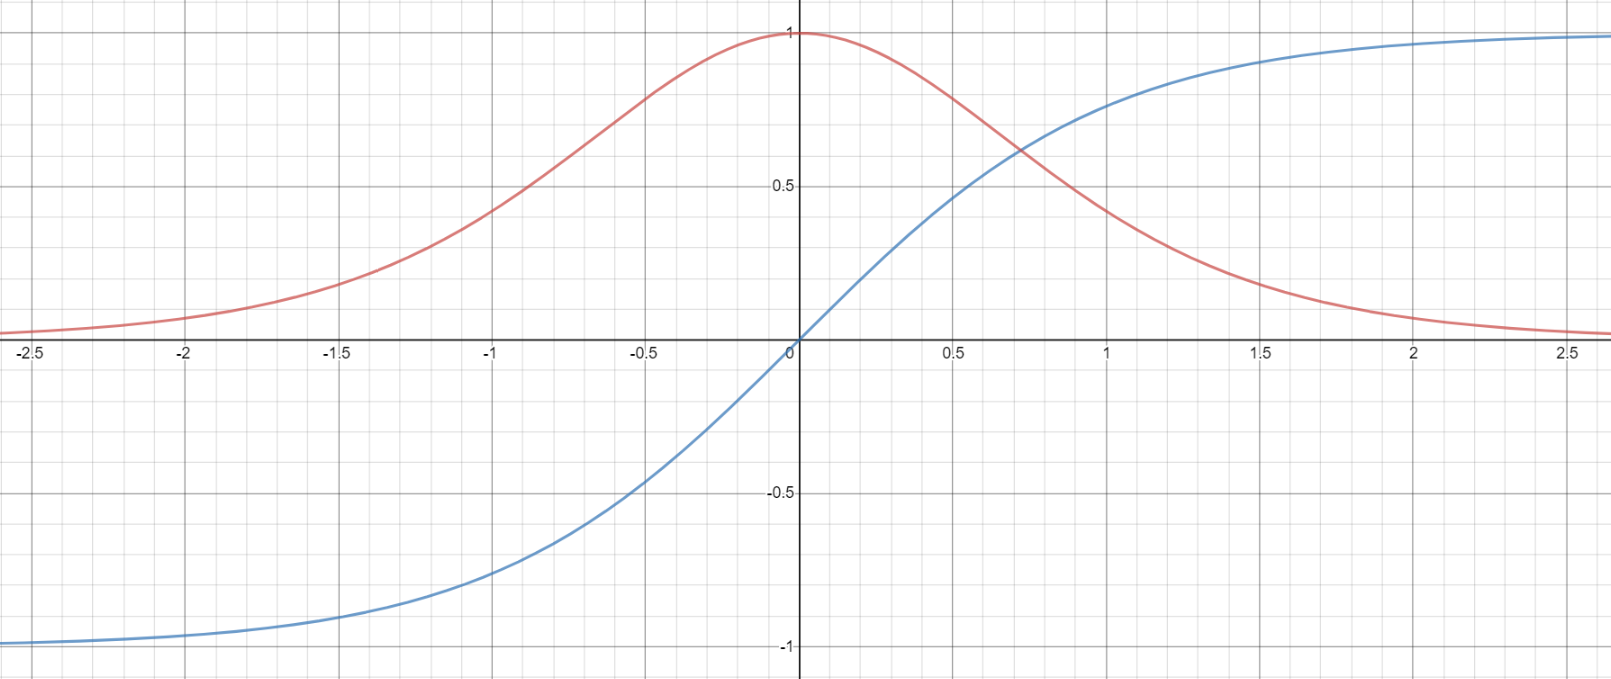
\includegraphics[width=0.75\columnwidth]{chapter03/figure/Tanh.png}
        \caption{Đồ thị và đồ thị đạo hàm của hàm tanh.}
        \label{fig:Tanh}
		\centering
\end{figure}

Hàm tanh cũng có thể được biểu diễn bằng hàm sigmoid như sau:
\[tanh(x) = 2\sigma(2x) - 1\]

\subsection{Hàm ReLU}
$\indent$\textbf{Công thức:}
\[f(x) = max(0,x)\]
\begin{figure}[!h]
	\centering
		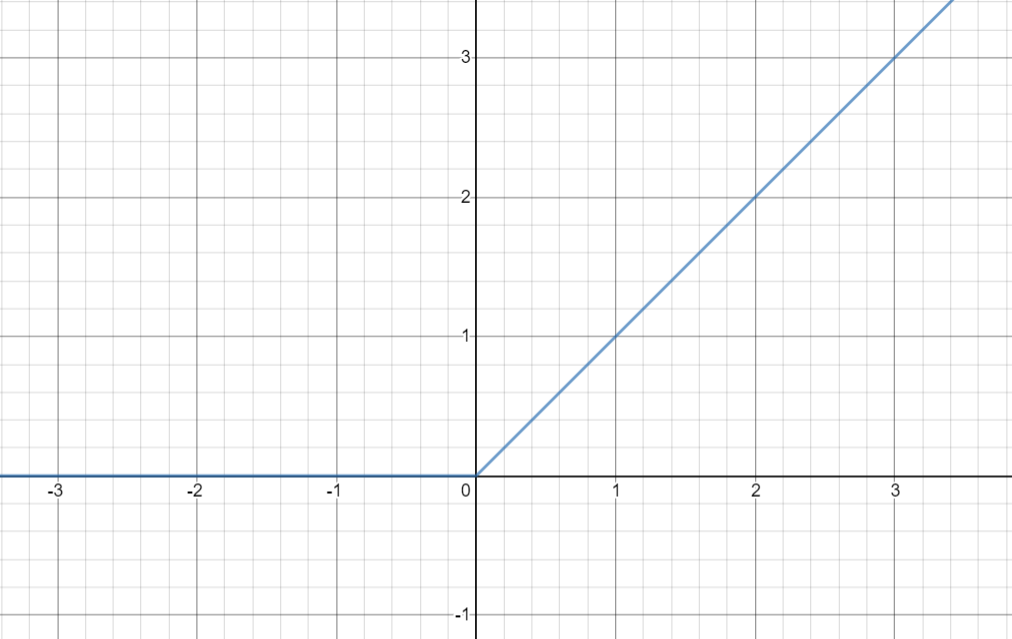
\includegraphics[width=0.75\columnwidth]{chapter03/figure/ReLU.png}
        \caption{Đồ thị của hàm ReLU.}
        \label{fig:ReLU}
		\centering
\end{figure}

Quan sát công thức và hình \ref{fig:ReLU}, dễ dàng nhận ra cách hoạt động của hàm ReLU là lọc ra các giá trị đầu vào nhỏ hơn 0. Đạo hàm của ReLU sẽ như sau:
\begin{equation}
    f'(x) = 
    \begin{cases}
      1 & \text{if } x > 0\\
      0 & \text{else}
    \end{cases}
\end{equation}

Như vậy, so với sigmoid và tanh, hàm ReLU sẽ không xuất hiện vấn đề triệt tiêu gradient. Tốc độ tính toán của hàm ReLU cũng sẽ nhanh hơn so với hai hàm trước đó. Tuy nhiên ReLU cũng tồn đọng một nhược điểm, với $x$ có giá trị nhỏ hơn 0, qua hàm  ReLU sẽ thu được kết quả bằng 0. Nếu giá trị của node bị chuyển thành 0 thì sẽ không có ý nghĩa ở lớp tiếp theo và các hệ số tương ứng từ node đấy cũng không được cập nhật với gradient. Hiện tượng này gọi là \textit{Dying ReLU}.

\subsection{Hàm leaky ReLU}
$\indent$\textbf{Công thức:} 
\[f(x) = max (0.01x,x)\]
$\indent$Leaky ReLU là một cố gắng trong việc loại bỏ Dying ReLU. Thay vì luôn trả về giá trị bằng 0 cho các giá trị âm, leaky ReLU tạo một đường xiên có độ dốc nhỏ như hình \ref{fig:leakyReLU}.
\begin{figure}[!h]
	\centering
		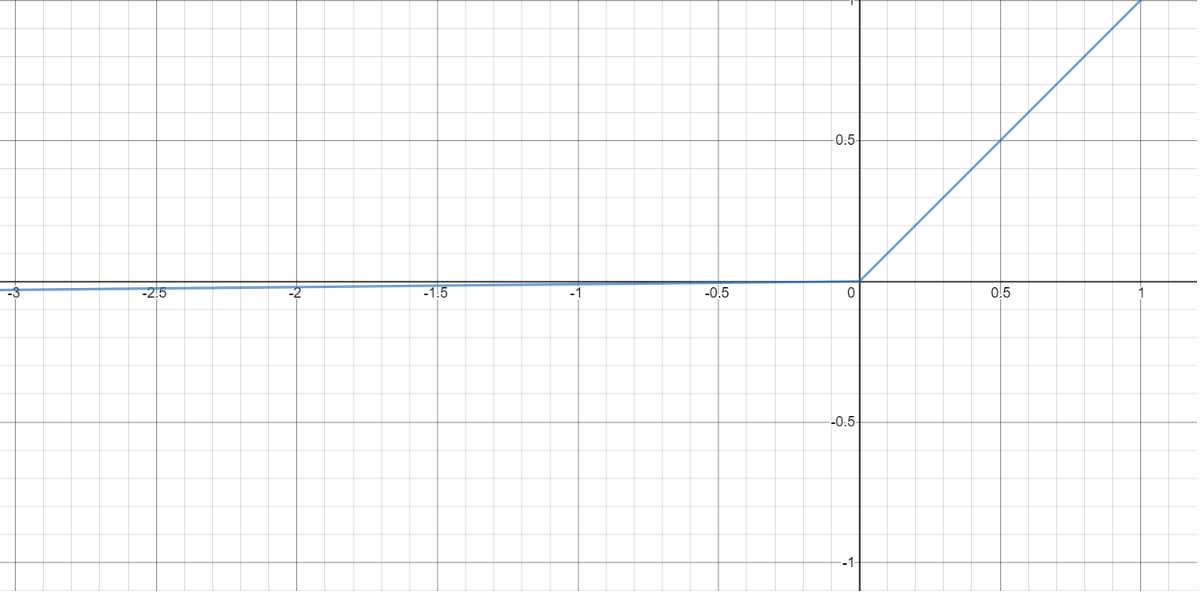
\includegraphics[width=0.75\columnwidth]{chapter03/figure/leakyReLU.png}
        \caption{Đồ thị của hàm leaky ReLU.}
        \label{fig:leakyReLU}
		\centering
\end{figure}

Leaky ReLU cũng có một biến thể khác là PReLU: $f(x) = max(\alpha x,x)$ với $\alpha$ sẽ được chọn trong quá trình học.
%%%%%%%%%%%%%%%%%%%%%%%%%%%%%%%%%%%%%%%%%%%%%%%%%

\section{Biểu diễn Neural Network như là vector và ma trận}
Chúng ta đã có những khái niệm về neural network qua những phần trước. Tuy nhiên, làm sao để máy tính có được bộ não với những neuron như vậy thì phần này sẽ đi giải đáp những vấn đề  đó.

\subsection{Làm sao biểu diễn được neural network}
Chúng ta xem xét mạng neural network gồm 3 layer như sau: 
\begin{figure}[!h]
	\centering
		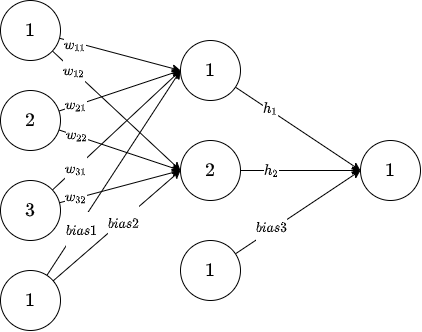
\includegraphics[width=0.5\columnwidth]{chapter03/figure/weight(1).png}
        \caption{Mạng neural network gồm 3 layer.}
        \label{fig:weight}
		\centering
\end{figure}

Dựa theo hình trên, với $f$ là hàm activation chúng ta sẽ thấy rằng:
\begin{center}
$h_{1} = f(in_{1}*w_{11}+in_{2}*w_{21}+in_{3}*w_{31}+bias_{1})$\\
$h_{2} = f(in_{1}*w_{12}+in_{2}*w_{22}+in_{3}*w_{32}+bias_{2})$\\
$out = f(h_{1}*w_{11}+h_{2}*w_{21}+bias_{3})$\\
\end{center}

Bằng một cách suy nghĩ đơn giản, chúng ta có thể lưu các giá trị $w_{i}$ vào một mảng hay một vector và duyệt tuần tự. Nhưng chúng ta nên sống chậm lại để để ý rằng, với mỗi perceptron nó sẽ được tính bằng cách lấy giá trị đầu ra của layers trước đó hoặc là giá trị input ban đầu (gọi chung là input) nhân với trọng số của nó nối với input hay nói theo kí hiệu toán học sẽ như sau:
\begin{center}
    $h_{i} = f(\sum_{j=1}^{num\_input} in_{j}*w_{ji}+bias_{i})$ (1)
\end{center}

Trong đó, $num\_input$ chính là số lượng input để tính toán trong tầng hiện tại. Nếu ai đã quen với việc tính toán ma trận thì sẽ thấy công thức này giống như việc nhân 2 ma trận với nhau.

Thật vậy, mỗi đầu ra của một perceptron là một con số (scalar) và mối quan hệ giữa 2 tầng liên tiếp là như nhau nên ở đây không mất tình tổng quát chúng ta chỉ xét riêng trường hợp với 2 tầng (nhìn hình minh họa).
\begin{figure}[!h]
	\centering
		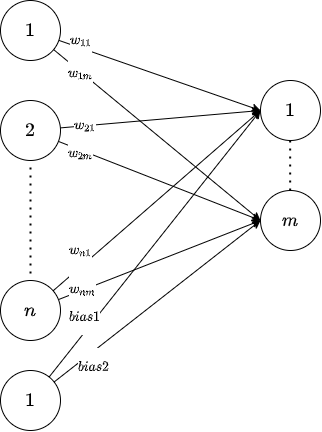
\includegraphics[width=0.5\columnwidth]{chapter03/figure/FC.png}
        \caption{Hai layer liên tiếp nhau.}
        \label{fig:FC}
		\centering
\end{figure}

Với hình trên, nếu chúng ta biểu diễn input thành 1 vector hay nói cách khác là một ma trận $X_{nx1}$. Ta sẽ xây dựng ma trận trọng số $W$ tương ứng với n hàng, m cột với $w_{ij}$ là trọng số từ input $i$ nối với một output $j$.

Dựa theo công thức ở (1), chúng ta có thể thấy rằng chỉ cần lấy cột thứ $i$ ra làm vector để nhân với vector trong ma trận cột $X$ và áp dụng activation thì ta sẽ có kết quả của perceptron thứ $i$. Do đó, việc còn lại để tính nhanh đó là ta chuyển vị ma trận trọng số $W_{nxm}$ thì sẽ trở về môn Đại số tuyến tính thân quen. Nếu lúc này chúng ta xét $h_{mx1}$ là ma trận của các perceptron đầu ra thì ta sẽ có công thức như sau:
\begin{center}
    $h = f(W^{T}*X+b)$
\end{center}

Cách biểu diễn neural network dưới dạng ma trận như thế này rất hữu ích trong việc tính toán khi thực hiện các phép lan truyền xuôi và lan truyền ngược.

\subsection{Cách biểu diễn lan truyền xuôi và lan truyền ngược}
\subsubsection{Lan truyền xuôi }
Lan truyền xuôi là quá trình tính toán thông qua các tầng ẩn mà dữ liệu đầu vào được cho ra kết quả trong mô hình. Ta kí hiệu mỗi tầng $i$ trong mạng được cấu tạo từ 3 phần đó là input $X^{(i)}$, ma trận trọng số $W^{(i)}$ và hàm activation $f^{(i)}$ , trong đó, output của tầng này sẽ là input của tầng tiếp theo. Xem xét hình minh họa dưới đây cho quá trình lan truyền xuôi.
\clearpage
\begin{figure}[!h]
	\centering
		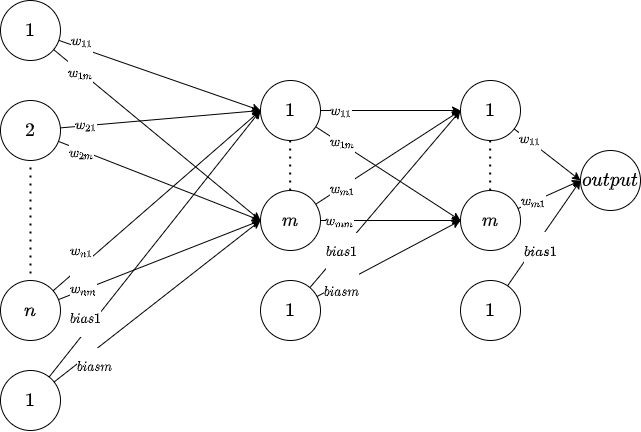
\includegraphics[width=0.75\columnwidth]{chapter03/figure/ltx.png}
        \caption{Lan truyền xuôi}
        \label{fig:ltx}
		\centering
\end{figure}

Như chúng ta thấy trong hình mạng gồm 4 layers (1 input layer, 2 hidden layer và 1 output layer).
\begin{center}
    $X^{(1)} = f^{(1)}(W^{(1)T}*Input+b^{(1)})$\\
    $X^{(2)} = f^{(2)}(W^{(2)T}*X^{(1)}+b^{(2)})$\\
    $Output = f^{(3)}(W^{(3)T}*X^{(2)}+b^{(3)})$\\
\end{center}

Với cách tính này, thì chúng ta có thể mở rộng một cách tông quát với 1 input layer, n hidden layer và 1 output layer như sau:
\begin{center}
    $X^{(1)} = f^{(1)}(W^{(1)T}*Input+b^{(1)})$\\
    $X^{(i)} = f^{(i)}(W^{(i)T}*X^{(i-1)}+b^{(i)})$, $i=\overline{2,n}$\\
    $Output = f^{(n)}(W^{(n)T}*X^{(n)}+b^{(n+1)})$\\
\end{center}

Nhìn chung, vấn đề lan truyền xuôi cũng không quá phức tạp khi đã có đại số tuyến tính can thiệp vào.

\subsubsection{Lan truyền ngược}
Lan truyền ngược là quá trình cập nhật lại cái trọng số để tìm ra bộ trọng số phù hợp để làm mô hình cho bài toán cần giải quyết. Khác với lan truyền xuôi khi sử dụng hàm activation, lan truyền ngược dựa trên việc tính đạo hàm để cho ra kết quả.

Để cập nhật được trọng số, thì chúng ta cần có hàm loss giả sử được định nghĩa là $J$ và để dễ cho quá trình tính toán, chúng ta sẽ kí hiệu thêm biểu thức sau:
\begin{center}
    $z^{(i)}=W^{(i)T}*X^{(i)}+b^{(i)}$
    $a^{(i)} = f(z^{(i)})$
\end{center}

Các kí hiệu này được biểu diễn như hình sau. Để đỡ rối khi nhìn, xin phép chỉ kí hiệu tượng trưng các đường cần thiết, thực tế sẽ mỗi perceptron ở layer trước phải nối hết với các perceptron layer sau.
\begin{figure}[!h]
	\centering
		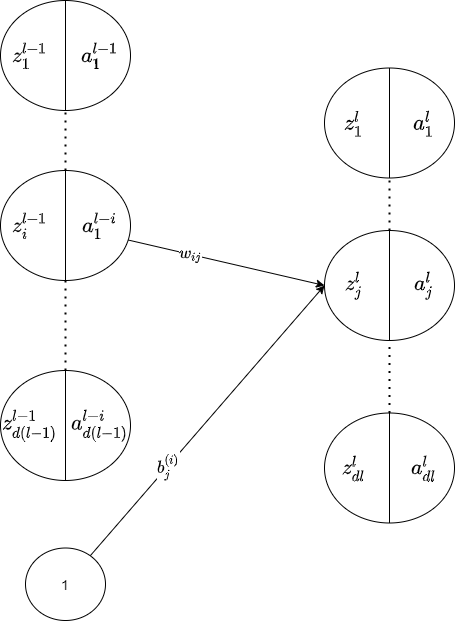
\includegraphics[width=0.5\columnwidth]{chapter03/figure/ltn.png}
        \caption{Đồ thị minh họa lan truyền ngược.}
        \label{fig:ltn}
		\centering
\end{figure}

Tiếp theo, chúng ta sẽ có được gradient của các trọng số ở từng layer l như sau:
\begin{center}
        $\frac{\partial J}{\partial w^{(l)}_{ij}} = \frac{\partial J}{\partial z_{j}^{(l)}} * \frac{\partial z_{j}^{(l)}}{\partial w^{(l)}_{ij}}=e^{(l)}_{j} * a_{i}^{(l-1)}$\\
\end{center}

với
\begin{center}
        $e^{(l)}_{j} = \frac{\partial J}{\partial z_{j}^{(l)}}=\frac{\partial J}{\partial a_{j}^{(l)}}*\frac{\partial a_{j}^{(l)}}{\partial z_{j}^{(l)}}$\\
        $=(\sum_{k=1}^{d^{(l+1)}} \frac{\partial J}{\partial z_{k}^{(l+1)}}*\frac{\partial z_{j}^{(l)}}{\partial a_{j}^{(l)}})f'(z^{(l)}_{j})$\\
        $=(w^{(l+1)}_{j:}*e^{(l+1)})f'(z^{(l)}_{j})$
\end{center}

Trong đó $e^{(l+1)} = [e_{1}^{(l+1)},e_{2}^{(l+1)},...,e_{d(l+1)}^{(l+1)}]^{T}$ và $w_{j:}^{(l+1)}$ là toàn bộ phần tử hàng thứ $j$ của ma trận $W^{(l+1)}$. Tổng xuất hiện trong công thức trên thể hiện việc $a_{j}^{(l)}$ đóng góp vào việc tính các $z_{k}^{(l+1)}$.
Với cách làm tương tự, ta có:
\begin{center}
        $\frac{\partial J}{\partial b^{(l)}_{j}} =e^{(l)}_{j}$\\
\end{center}

Từ đây chúng ta có thể mở rộng ra cho cách biểu diễn bằng ma trận như các công thức sau:
\begin{center}
    $\frac{\partial J}{\partial W^{(l)}} = a^{(l-1)}e^{(l)T}$\\
    $e^{(l-1)} = W^{(l)T}e^{(l)}f'(z^{(l)})$\\
    $\frac{\partial J}{\partial b^{(l)}} = e^{(l)}$
\end{center}

\subsection{Vì sao lại biểu diễn bằng ma trận}
Để giải quyết cho câu hỏi này, hãy thử hiện thực các tính toán trong mạng neural mà không dùng đến ma trận:
\begin{lstlisting}
    J = 0
    for i = 1 to m:
        z[i] = b
        for j in range(len(w)):
            z[i] += w[j]*x[i][j] 
        a[i] = Sigmoid(z[i])
        J += -[y[i]*log(a[i]) + (1-y[i])*log(1-y[i])]
        dz[i] = a[i] - y[i]
        for j in range(len(w)):
            dw[j] += x[i][j]*dz[i]
    J = J / m
    for j in range(len(w)):
        w[j] = w[j] - alpha*dw[j]/m
\end{lstlisting}

Và hiện thực các tính toán có sử dụng ma trận:
\begin{lstlisting}
    import numpy as np 
    
    Z = np.dot(w.T,X) + b
    A = Sigmoid(Z) #1
    dZ = A - Y
    dW = (1/m) * X * dZ.T
    dB = (1/m) * np.sum(dZ)
    W = W - alpha * dW
    b = b - alpha * dB
\end{lstlisting}

Có thể thấy, việc hỗ trợ tính toán bằng ma trận giúp ích rất nhiều trong quá trình hiện thực. Đó cũng là lý do tại sao những ngôn ngữ có hỗ trợ tính toán ma trận như Python được sử dụng phổ biến trong hiện thực mạng neural. Một lưu ý nữa được rút ra từ ví dụ trên là các nút ở cùng một tầng thì phải có cùng một hàm activation để việc áp dụng hàm activation (dòng 1) cũng ma trận hóa và trở nên dễ dàng hơn.

\subsection{Kỉ nguyên mới của neural network} 
Sau khi đã đi qua những lý thuyết của neural network thì chúng ta đã thấy được sức mạnh của phương pháp này. Tuy nhiên, đã có thời gian neural network không được sử dụng nhiều và chìm trong màn đêm. Vấn đề nằm ở chỗ, việc tính toán ma trận quá sức phức tạp và Central Processing Unit(CPU) và cả Graphics Processing Unit(GPU) thời bấy giờ chưa thể đảm nhận được công việc này. Tuy nhiên, sau khi phần cứng phát triển vượt bậc thì đã mở ra kỉ nguyên mới cho neural network.

Ngày nay, khi nhắc đến việc huấn luyện mạng neural network, người ta thường nghĩ ngay đến việc huấn luyện trên GPU. Nhưng tại sao CPU và GPU đã phát triển nhưng GPU lại chiếm ưu thế hơn trong việc lựa chọn để huấn luyện?

Để trả lời câu hỏi này, chúng ta quay lại việc lan truyền xuôi và lan truyền ngược sử dụng ma trận. Có thể nói rằng việc biểu diễn neural network bằng ma trận là cách tốt nhất trong hiện tại. Do đó, phần cứng nào có thể lưu trữ những con số dưới dạng ma trận đều có thể đảm nhận được nhiệm vụ tính toán và biểu diễn neural network tốt nhất.

Nói đến đây, ắt hẳn chúng ta đã biết tại sao GPU đã có sức ảnh hưởng mạnh mẽ đến neural network. GPU được dùng để biểu diễn hình học đồ họa máy tính, mà đồ họa máy tính được cấu thành từ ma trận pixel nên việc xử lý này không khác gì xử lý ma trận trong neural network cả. Thêm vào đó, GPU ngày nay lại được xử lý đa luồng và tiếp nhận thông tin gấp nhiều lần CPU. Hãy tưởng tượng xem, để xử lý ma trận thì CPU phải duyệt qua các phần tử trong ma trận và thực hiện tính toán, chúng ta có thể lấy CPU nhiều core nhưng chắc chắn rằng cũng chỉ vài chục là nhiều. Trong khi đó, GPU có thê lập tức biến đổi ngay vector hay ma trận nhờ vào khả năng tính toán song song của mình. Đây cũng là lý do mà chúng ta phải dùng ma trận hóa ở phần trước để tính toán và cũng là lý do vì sao các framework về học sâu ngày nay \textbf{chỉ cho dùng 1 hàm activation cho mỗi tầng}.

\section{Kết chương}
 Qua chương này, chúng ta đã tìm hiểu và phân tích được cách thức hoạt động của mạng học sâu mà ngày nay được sử dụng ngoài thực tế. Ngoài ra, các vấn đề liên quan tới GPU và ma trận hóa cũng đã được trình bày để thấy được sự ảnh hưởng của phần cứng và sự hỗ trợ của ngôn ngữ khi chúng ta huấn luyện mạng học sâu để từ đó chúng ta có phương pháp lựa chọn phần cứng, ngôn ngữ và thiết kế mô hình mạng hợp lý để tối ưu năng suất nhất có thể.

\newpage
\section{Bài tập}
\begin{exer}
Cho mạng neural network như hình vẽ sau:
%%%%%%%%%%%%Chen hinh
\begin{figure}[!h]
	\centering
		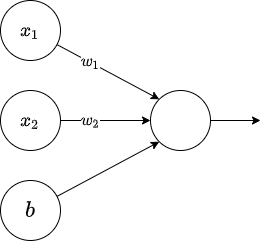
\includegraphics[width=0.5\columnwidth]{chapter03/figure/bai1.png}
        \caption{Mạng neural network một output.}
		\centering
\end{figure}\\
Biết rằng $w_{1} = w_{2} = w_{bias} = 0.25$, $x1=0.1, x2=0.2, bias= 1$ và output mong đợi là 1. Hãy tính output của mạng và các trọng số và bias mới(với hệ số học alpha là 0.1 và hàm lỗi là $CrossEntropy$) của mạng với các activation sau:
\begin{enumerate}
    \item Hàm activation là hàm $tanh$.
    \item Hàm activation là hàm $ReLU$.
\end{enumerate}
\end{exer}

\clearpage
\begin{exer}
Cho mạng neural network như hình vẽ sau:
%%%%%%%%%%%%Chen hinh
\begin{figure}[!h]
	\centering
		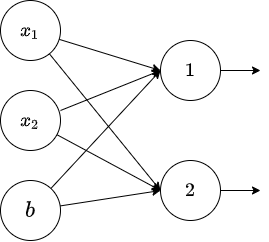
\includegraphics[width=0.5\columnwidth]{chapter03/figure/bai2.png}
        \caption{Mạng neural network hai output.}
        \label{sec3:bai2}
		\centering
\end{figure}

Biết rằng các trọng số và bias đều bằng $0.5$, $x1=0.1, x2=0.2$ và output 1, 2 mong đợi lần lượt là 0, 1. Hãy tính output của mạng và các trọng số và bias mới(với hệ số học alpha là 0.1 và hàm lỗi là $CrossEntropy$) của mạng với các activation sau:
\begin{enumerate}
    \item Hàm activation của output 1, 2 lần lượt là là hàm $tanh$, $ReLU$.
    \item Hàm activation output 1, 2 lần lượt là là hàm $tanh$, $tanh$.
\end{enumerate}
\end{exer}

\clearpage
\begin{exer}
Cho mạng neural network như hình vẽ sau:
%%%%%%%%%%%%Chen hinh
\begin{figure}[!h]
	\centering
		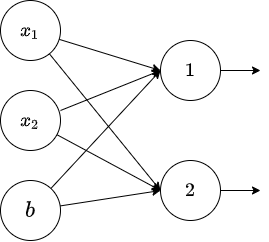
\includegraphics[width=0.5\columnwidth]{chapter03/figure/bai2.png}
        \caption{Mạng neural network hai output.}
		\centering
\end{figure}

Biết rằng các trọng số và bias đều bằng $0.5$, $x1=0.1, x2=0.2$ và output 1, 2 mong đợi lần lượt là 0, 1. Hãy dựa theo kiến thức của chương này, tìm ra các ma trận được tạo ra và dùng vectorize để tính toán thực hiện lan truyền xuôi.
\end{exer}